\chapter[Metodologia]{Metodologia}

\section{Metodologia de Desenvolvimento}

Para a concepção do trabalho haverá uma junção de diferentes metodologias ágeis. Essa abordagem tem como objetivo selecionar as melhores práticas de cada metodologia a fim de otimizar o desenvolvimento das tarefas que compõem a elaboração desse trabalho.  

Com o intuito de realizar um desenvolvimento mais produtivo, será utilizado alguns elementos da metodologia Scrum. Dessa forma, será organizado um \textit{Product Backlog} para executar e organizar as tarefas a serem desenvolvidas conforme suas prioridades. As \textit{Sprints} terão a duração de uma semana. No início da semana, as tarefas a serem realizadas na \textit{Sprint} serão organizadas no \textit{Sprint Backlog} e ao final da semana será analisado o que foi feito e os débitos para a \textit{Sprint} seguinte, além da possibilidade de mudança nas prioridades e na inserção de novas tarefas no \textit{Product Backlog}. 

Para melhorar o controle e visualização das tarefas a serem realizadas e assim otimizar o desenvolvimento, a agilidade e eficácia, será utilizada a metodologia KanBan com algumas modificações. As tarefas a serem desenvolvidas estarão representadas no formato de \textit{User Story}. Os cartões que farão parte do quadro terão o seguinte conteúdo: um identificador único, uma descrição da tarefa no padrão de sentença ``Eu, como <quem>, desejo <o que>'', sua categoria, as atividades a serem realizadas e a indicação da \textit{Sprint}.

O quadro KanBan será constituído por 5 diferentes colunas: \textit{Product Backlog}, \textit{Sprint Backlog}, Em Progresso, Revisão e Fechadas. A Figura \ref{quadroKanBan} apresenta um exemplo de como o quadro KanBan será organizado para o desenvolvimento do trabalho. 

\begin{figure}[h]
	\centering
	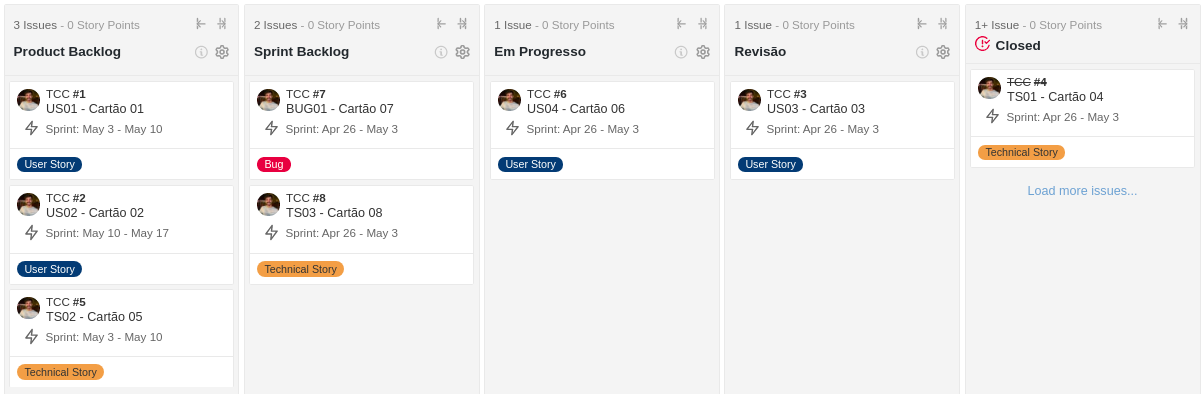
\includegraphics[keepaspectratio=true,scale=0.375]{figuras/kanban.png}
	\caption{Quadro KanBan representado na ferramenta \href{https://www.zenhub.com/}{ZenHub}}
	\label{quadroKanBan}
\end{figure}

Na coluna \textit{Product Backlog} estarão os cartões com todas as funcionalidades que o trabalho deve possuir, onde os de maiores prioridades ficarão em cima da pilha. Nessa coluna, \textit{bugs} e melhorias poderão ser adicionados durante o desenvolvimento do trabalho. Na coluna \textit{Sprint Backlog} estarão o conjunto de tarefas planejadas para serem executadas durante a semana da \textit{Sprint}. A coluna Em Progresso possuirá as tarefas que estão sendo realizadas no momento. Já a Revisão conterá os cartões que estiverem passado por um processo de revisão para assim então irem para a coluna de Finalizados, que possuirá um histórico de todos as tarefas feitas.

A fim de desenvolver um código com boa qualidade, é imprescindível a adoção de boas práticas de programação, dessa forma, a metodologia \textit{Extreme Programming} define alguns elementos que serão utilizados. O primeiro é a adoção de uma folha de estilo para que se possa realizar padronizações de codificação e o segundo é a realização de refatorações do código.

\section{Políticas do Repositório}

Todo o Software será armazenado na plataforma \href{https://github.com/}{GitHub} em um repositório aberto. As tarefas a serem desenvolvidas serão cadastradas como \textit{issues} no GitHub e utilizadas como cartões no quadro KanBan de forma visual pela ferramenta ZenHub.

O repositório do projeto seguirá o fluxo de trabalho conhecido como GitFlow, conforme a Fig. \ref{gitflow} e possuirá as seguintes ramificações: a \textit{Main} que será a ramificação principal e que possuirá a versão estável do código; a \textit{Develop} que será uma ramificação da \textit{Main} e servirá para integração de recursos; a \textit{Feature} será dedicada para a criação de novas funcionalidades e após finalizada e revisada será integrada à \textit{Develop}; a \textit{Release} é uma ramificação da \textit{Develop} e será criada ao final de uma \textit{Sprint}, quando estiver pronta para o lançamento, ela deve ser mesclada com a \textit{Main} e com a \textit{Develop}; a \textit{Hotfix} deve ser criada sempre que algum erro em produção for detectado.  

\begin{figure}[h]
	\centering
	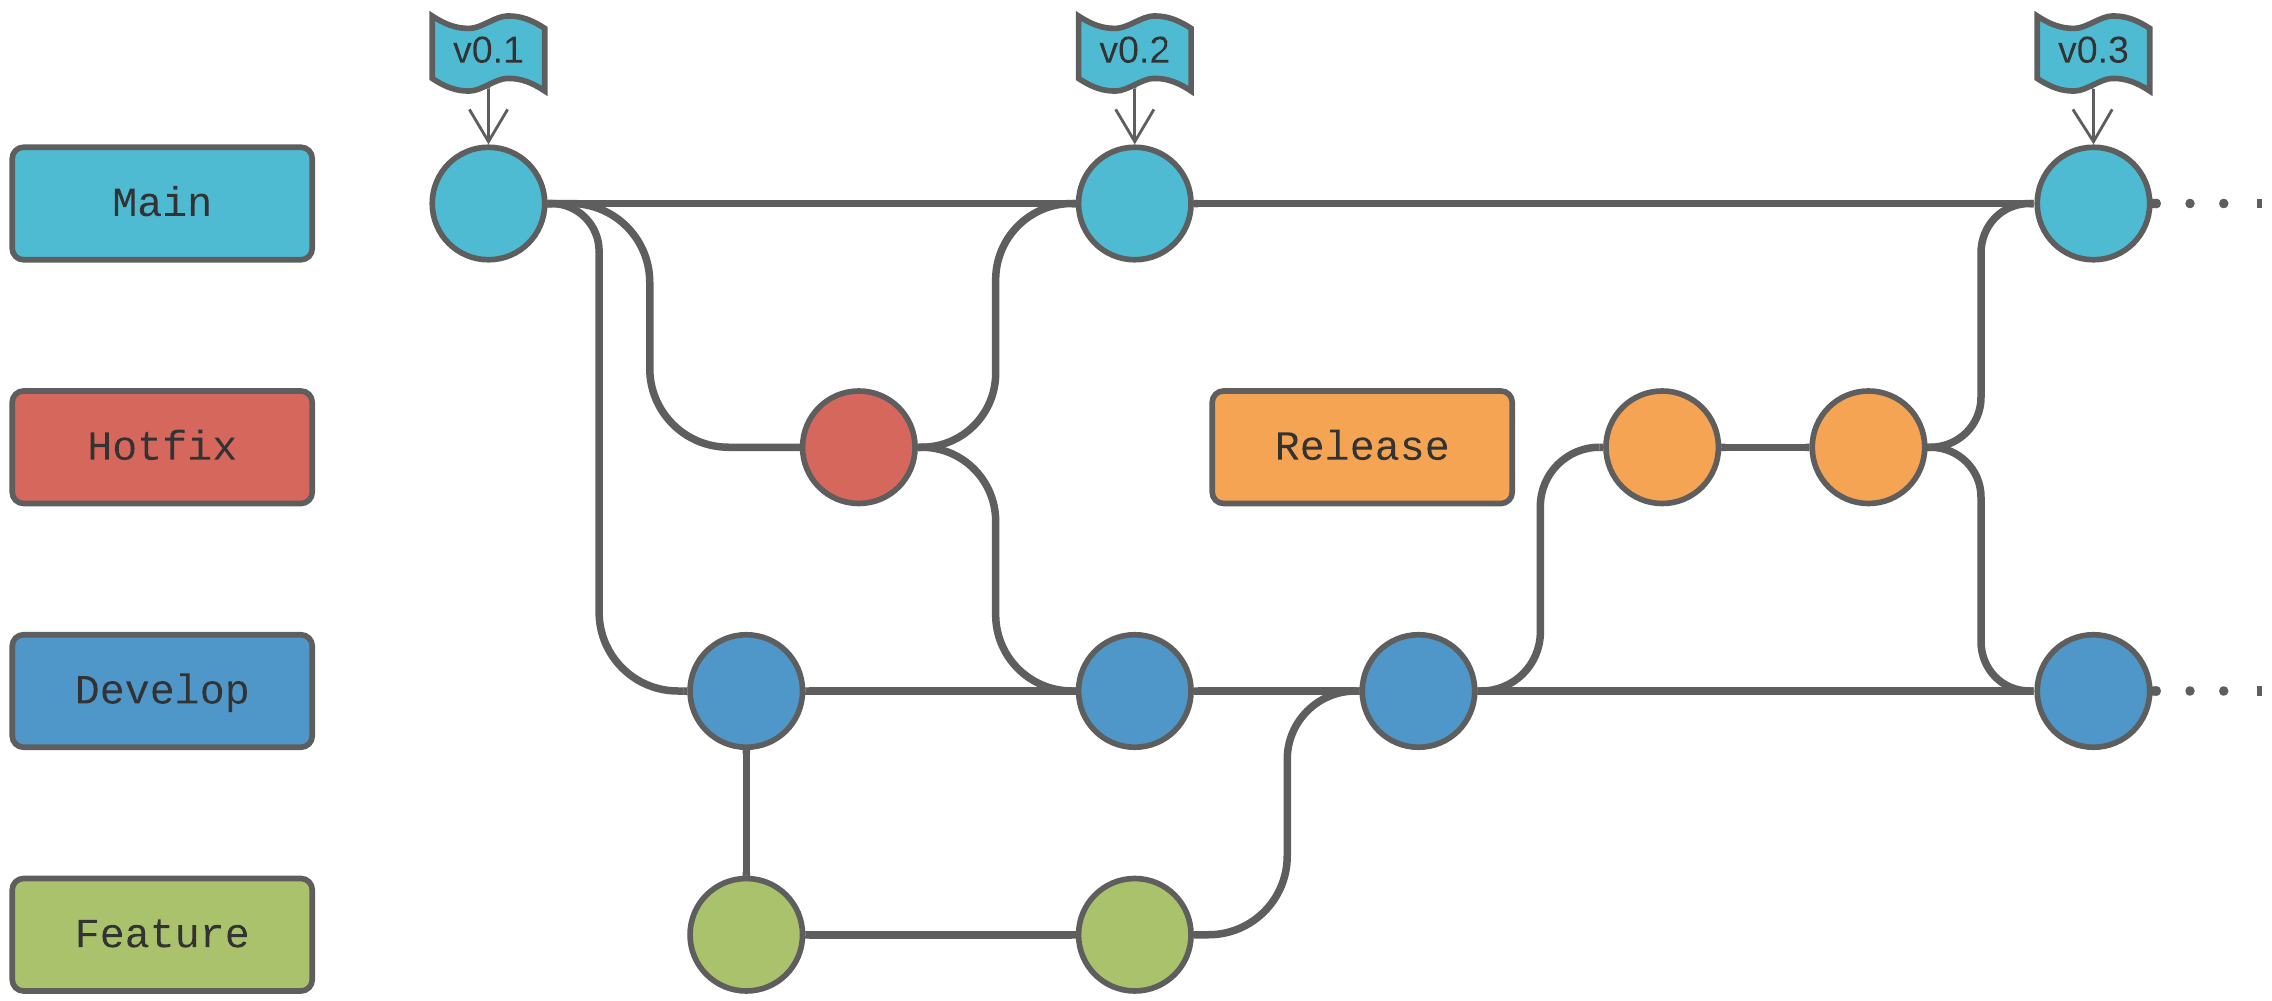
\includegraphics[keepaspectratio=true,scale=0.18]{figuras/git flow.png}
	\caption{Fluxo de trabalho segundo o GitFlow}
	\label{gitflow}
\end{figure}

Os \textit{commits} deverão descrever sucintamente o que foi feito, serem atômicos, serem escritos no gerúndio, em inglês, e deverão ser identificados pelo código da \textit{issue} a que se refere, como no seguinte exemplo: ``\#1 - Creating project''.

\section{Linguagens e Ambiente de Desenvolvimento}

Para a criação do módulo será utilizada a linguagem de programação Dart, uma linguagem que tem se popularizado devido ao \textit{framework} Flutter, que permite o desenvolvimento de aplicações nativas para web, mobile e desktop. Nessa linguagem de programação, foi verificada a falta de uma biblioteca que implementasse os algoritmos Ed448 e Ed521, devido a isso, essa linguagem será utilizada para a implementação do módulo que realizará a assinatura e verificação de acordo com o algoritmo EdDSA. A fim de realizar uma prova de conceito, será feita uma validação cruzada com uma biblioteca mais madura na linguagem Python. 

Tanto para o estudo dessas linguagens quanto para a elaboração do módulo mencionado, será utilizada o editor de código \textit{Visual Studio Code}, uma ferramenta de desenvolvimento produzida pela Microsoft.

\section{Integração Contínua e Implantação Contínua}

A integração contínua e a implantação contínua será realizada por meio do \href{https://docs.github.com/pt/actions}{GitHub Actions}, dessa forma, será possível executar um fluxo de trabalho totalmente automático, que analisará a qualidade e a padronização do código, realizará testes, empacotará os módulos e os publicará no sistema de gerenciamento de pacotes pub.dev.

Assim que um \textit{Pull Request} for aberto, será analisado a qualidade e a padronização do código pela ferramenta Linter e um fluxo de testes será realizado e caso sejam aprovados, um \textit{merge} do código estará liberado para ser feito na ramificação \textit{Main}. Assim que o \textit{merge} for feito, uma nova versão do pacote será publicado  

